\apendice{Especificación de diseño}
\begin{comment}
\section{Introducción}

\section{Diseño de datos}

\section{Diseño procedimental}

\section{Diseño arquitectónico}
\end{comment}

\section{Diseño de las interfaces}

En esta sección se explicarán las diferentes interfaces de los productos realizados en este trabajo fin de grado.

\subsection{\textit{Jupyter Notebook} para el reconomiento de caras}

Durante el primer mes se trabajo en un \textit{Jupyter Notebook} que trataba de reconocer caras mediante un clasificador junto a un extractor de características, como ya hemos explicado en secciones anteriores. Con este \textit{Jupyter Notebook} se trataba de facilitar la evaluación del rendimiento de los clasificadores y el cambio de las distintas variables de manera interactiva. 

Por lo tanto, la interfaz de este \textit{Jupyter Notebook} no ha sido trabajada para su uso por parte del usuario. Sino que fue creada para un uso más de experimentación. Es por ello que la interfaz no tiene un buen grado de usabilidad como podemos observar en la figura \ref{fig:C.5.1}.

\begin{figure}[h]
\centering
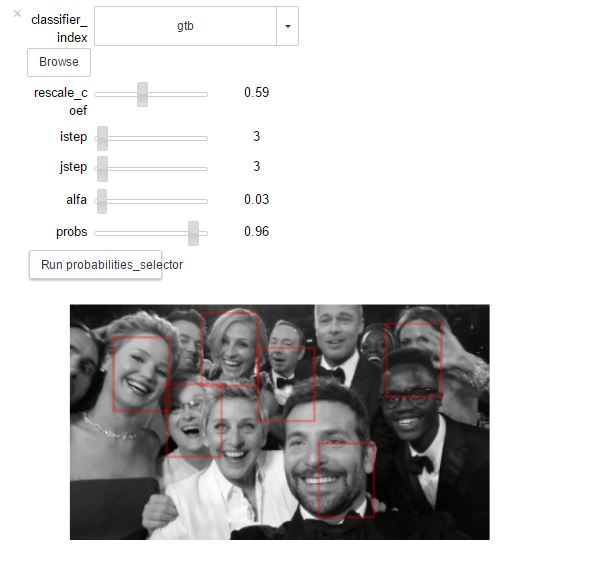
\includegraphics[width=0.99\textwidth]{reconocimiento_de_caras_notebook_v1}
\caption{\textit{Jupyter Notebook} para el reconomiento de caras}
\label{fig:C.5.1}
\end{figure}

\subsection{Etiquetador de imágenes}

La interfaz del etiquetador de imágenes ha sido desarrollada partiendo del prototipo mostrado en la ilustración \ref{fig:C.5.2}. Tratando de crear una interfaz lo más simple e intuitiva para el usuario.

\begin{figure}[h]
\centering
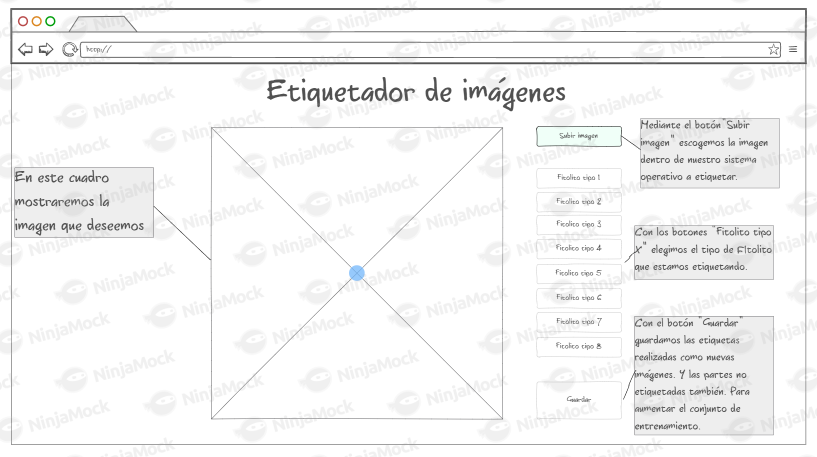
\includegraphics[width=0.99\textwidth]{protototipo_etiquetador_de_imagenes}
\caption{Prototipo del etiquetador de imágenes}
\label{fig:C.5.2}
\end{figure}

El resultado tras la implementación de este producto es el mostrado en la \ref{fig:C.5.3}. Obteniendo una interfaz muy similar a la prototipada en un principio. Pero añadiendo algún elemento más, para facilitar su uso por parte del usuario.

\begin{figure}[h]
\centering
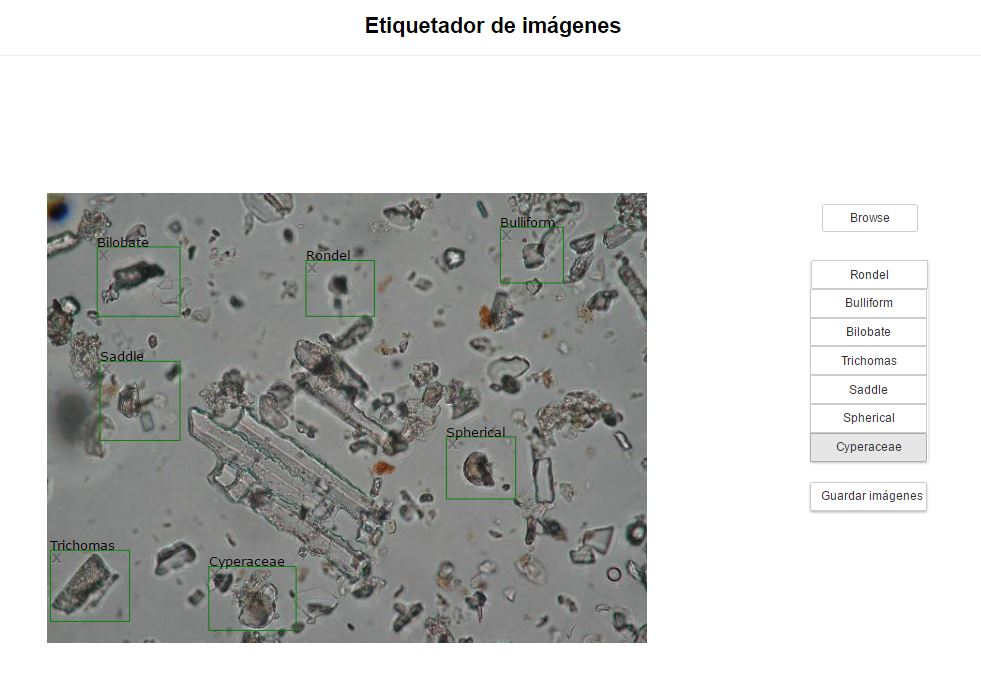
\includegraphics[width=0.99\textwidth]{etiquetador_de_imagenes_v1}
\caption{Etiquetador de imágenes}
\label{fig:C.5.3}
\end{figure}